\documentclass[11pt]{beamer}
\usetheme{Warsaw}
\usepackage[utf8]{inputenc}
\usepackage{amsmath}
\usepackage{amsfonts}
\usepackage{amssymb}
\usepackage{graphicx}
\usepackage[export]{adjustbox}
\usepackage{algorithm,algpseudocode}
\author{Brendan Benshoof}
\title{Survey of Parallel Convex Hull Algorithims}
%\setbeamercovered{transparent} 
%\setbeamertemplate{navigation symbols}{} 
%\logo{} 
%\institute{} 
%\date{} 
%\subject{} 
\begin{document}
\setcounter{tocdepth}{3}
\begin{frame}
\titlepage
\end{frame}

\section{Overview}
\subsection{Quick Review}

\begin{frame}{this is a Convex Hull}
  % - A title should summarize the slide in an understandable fashion
  %   for anyone how does not follow everything on the slide itself.
  \begin{itemize}
  \item
    A convex hull is a sub-set of points that describe a hull that contains a convex set and all the points as part of that set.
  \item
  	A convex Hull is often compared to stretching a rubber band around a set of points.
  \item
   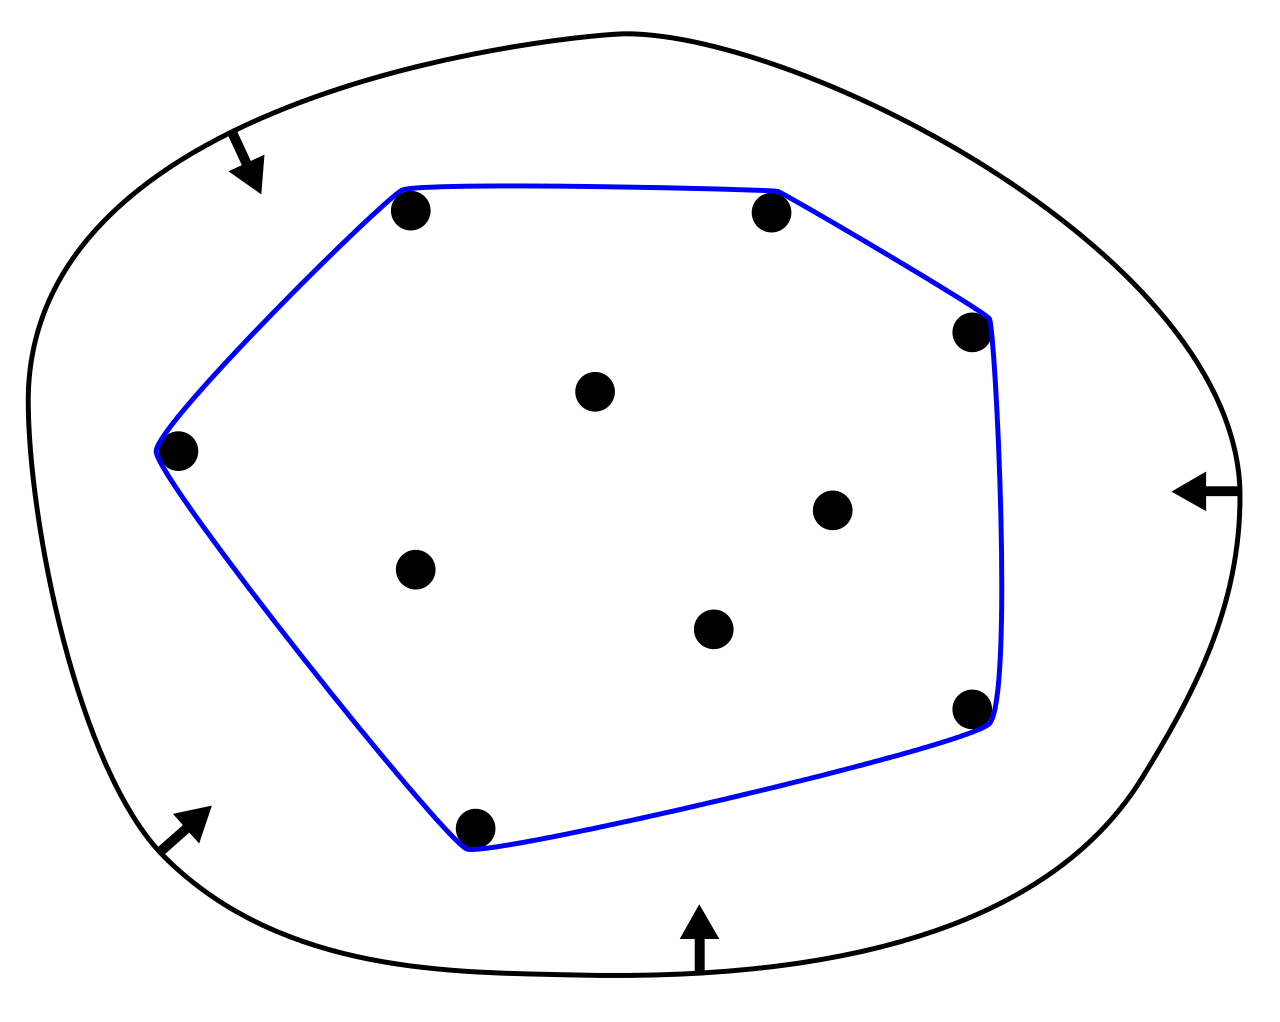
\includegraphics[width=.5\linewidth]{imgs/convex_hull.png}
By Maksim (original); en:User:Pbroks3 (redraw) [Public domain], via Wikimedia Commons
%  \caption{A non-convex set}
  \end{itemize}
\end{frame}
\begin{frame}{Division of Works}

Works examined fall roughly into 3 main approaches
\begin{itemize}
\item{ Divide and Conquer Methods}
\begin{itemize}
\item{``Efficient parallel solutions to some geometric problems.''}
\item{``Efficient parallel convex hull algorithms.''}
\item{ ``Scalable 2d convex hull and triangulation algorithms for coarse grained multicomputers.''}

\end{itemize}
\item{ Qhull derived methods}
\begin{itemize}
\item{``The quickhull algorithm for convex hulls.''}
\item{ ``Parallel implementation of 3D convex-hull algorithm.''}
\item{``Fast two dimensional convex hull on the GPU.''}
\item{``CudaHull: Fast parallel 3D convex hull on the GPU''}
\end{itemize}
\item{ Sampling Based Methods}
\begin{itemize}
\item{``A randomized parallel 3D convex hull algorithm for coarse grained multicomputers.''}
\item{ ``Fast randomized parallel methods for planar convex hull construction.''}
\item{``Parallel algorithms for higher-dimensional convex hulls.''}
\end{itemize}

\end{itemize}

\end{frame}




\section{Divide and Conquer}
\begin{frame}{Overview}
Divide and Conquer methods were the one of the first approaches considered for parallel computers.
They involve dividing the problem space into a number of discrete subspaces, solve for convex hulls locally, then merging the results.
\end{frame}

\begin{frame}{Efficient parallel solutions to some geometric problems}
\begin{itemize}
\item{Atallah, Mikhail J., and Michael T. Goodrich.}
\item{1986}
\end{itemize}
This is the approach to parallel convex hulls described in our textbook.
This paper presents a $O(log(n))$ time approach to with $O(n)$ processors

\end{frame}

\begin{frame}{Efficient parallel convex hull algorithms.}
\begin{itemize}
\item{Miller, Russ, and Quentin F. Stout.}
\item{1988}
\end{itemize}
Miller et al shows algorithms for preforming the convex hull operation given pre-sorted input on a variety of parallel architectures: a hypercube, pyramid,
tree, mesh-of-trees, mesh with reconfigurable bus, EREW PRAM, and a modified AKS network.

\end{frame}



\begin{frame}{Scalable 2d convex hull and triangulation algorithms for coarse grained multicomputers.}
\begin{itemize}
\item{Afonso Ferreira, Andrew Rau-Chaplin and Stkphane Ukda}
\item{1999}
\end{itemize}
This paper presents application of the algorithm described by Atallah et al onto a ``Course Grained'' computer model. This shows the algorithm can be preformed while preserving it's cost on a variety of limited communication systems.

\end{frame}





\section{Quickhull}

\begin{frame}{The quickhull algorithm for convex hulls.}

\begin{itemize}
\item{C. Bradford Barber, David P. Dobkin, and Hannu Huhdanpaa. }
\item{1996}
\end{itemize}
Quickhull was initially presented as a sequential computing algorithm. As a sequential algorithm, it was analytically unimpressive $O(nlog(n))$ time on par with the known performance bound. However, it proved to be highly parallelizable for GPU machines and conceptually extensible into higher dimensions. It aggressively eliminates internal nodes from the set of candidate points and provides a problem space that does not require inter-process communication.

Qhull is a popular open source library implementing the QuickHull algorithm.
\end{frame}




\begin{frame}{Fast two dimensional convex hull on the GPU.}
\begin{itemize}
\item{Srungarapu S., Reddy D.P., Kothapalli K. and Narayanan, P.J.}
\item{2011}
\end{itemize}
This paper provides initial implementation of 2D QuickHull in CUDA. It provides an $O(n\frac{log(p)}{p})$ time algorithim with $O(p)$ processors.
\end{frame}


\begin{frame}{CudaHull: Fast parallel 3D convex hull on the GPU.}
\begin{itemize}
\item{Ayal Stein, EranGeva, JihadEl-Sana}
\item{2012}
\end{itemize}
This paper provides implementation of 3D QuickHull for CUDA. They provide a $O(\frac{n}{p}log(n))$ time algorithm, with a $O(h)$ sequential cleanup setup (where $h$ is the number of points on the convex hull) to provide a proper convex polytope description of the Hull (nontrivial in 3+ dimensions). 
\end{frame}

\section{Sampling Methods}
\begin{frame}{Overview}
Randomized sampling methods are based on applying parallel linear programming techniques to the convex hull problem. Most of these algorithms apply randomized searching methods that are not analytically guaranteed to be the correct solution. However these algorithms provide a likelihood of accuracy such that the answer can reasonably be expect to be correct.

This approach does not provide faster algorithms than the previous two approaches discussed and has added difficulty in implementation.

\end{frame}

\begin{frame}{Parallel algorithms for higher-dimensional convex hulls.}
\begin{itemize}
\item{Amato, Nancy M., Michael T. Goodrich, and Edgar A. Ramos.}
\item{1994}
\end{itemize}
This paper provides a EREW PRAM model for solving high dimension convex hulls using probabilistic linear programming methods in $O(log(n))$ time with $O(nlog(n)+n^{\frac{d}{2}})$ work.
\end{frame}

\begin{frame}{A randomized parallel 3D convex hull algorithm for coarse grained multicomputers.}
\begin{itemize}
\item{Dehne, Frank and Deng, Xiaotie and Dymond, Patrick and Fabri, Andreas and Khokhar, Ashfaq A.}
\item{1995}
\end{itemize}
Dehne et al supplies a high-probability of accuracy algorithm for 3d convex hull on EREW PRAM of O(log(n)) time by converting the convex hull problem into a linear program. The linear program solution only provides the set of points on the hull and a linear time method of building the polytope is utilized.

\end{frame}


\begin{frame}{Fast randomized parallel methods for planar convex hull construction.}
\begin{itemize}
\item{Ghouse, Mujtaba R., and Michael T. Goodrich}
\item{1997}
\end{itemize}
Ghouse et al proposes the O(1) and O(nlog(n)) work algorithm for CRCW PRAM. The convex hull problem is presented as a linear programming problem and solved using probabilistic parallel linear programming techniques.

\end{frame}





\end{document}